\section{Metodi di analisi dell'errore}
Parliamo ora delle tecniche per l'analisi dell'errore. La continuità della funzione implica che il problema sia
\emph{ben posto}. Dalla relazione
\[
	\ein = \frac{f(\tx) - f(x)}{f(x)} =
	\frac{f(\tx) - f(x)}{\tx - x} \frac{x}{f(x)} \frac{\tx - x}{x}
\]
si ricava che la \emph{differenziabilità} di $f(x)$ è essenziale per il controllo dell'errore inerente. In
particolare se la funzione è \textbf{regolare}, ossia derivabile due volte con derivate continue, allora
vale
\[ f(\tx) = f(x) + f'(x) (\tx - x) + f''(\xi) \frac{(\tx - x)^2}{2} \]
ossia, lo sviluppo di Taylor di $f$ con resto in forma di Lagrange arrestato al secondo ordine intorno a
$\tx$ con $|\xi - x| \leq |\tx - x|$, da cui si ottiene
\begin{align*}
	f(\tx) - f(x) =              & f'(x) (\tx - x) + f''(\xi) \frac{(\tx - x)^2}{2} \\
	=                            & f'(x) \frac{\tx - x}{x} x +
	f''(\xi) \frac{(\tx - x)^2}{x^2} \frac{x^2}{2}                                  \\
	=                            & f'(x) \frac{\tx - x}{x} x +
	f''(\xi) \left( \frac{\tx - x}{x} \right)^2 \frac{x^2}{2}                       \\
	=                            & f'(x) \epsilon_x x +
	f''(\xi) \epsilon_x^2 \frac{x^2}{2}                                             \\
	\doteq                       & f'(x) \epsilon_x x                               \\
	\frac{f(\tx) - f(x)}{f(x)} = & \frac{f'(x)}{f(x)} \epsilon_x x
\end{align*}

\subsection{Coefficiente di amplificazione}
\begin{definition}
	La quantità
	\[ c_x = c_x (f) = \frac{f'(x)}{f(x)} \cdot x \]
	è detta \textbf{coefficiente di amplificazione} e fornisce una misura del condizionamento del problema.
\end{definition}

Più in generale possiamo dire che se $f : \Omega \to \R$ è definita su un insieme aperto di $\R^n$, differenziabile
due volte su $\Omega$ ed il segmento di estremi $\tx$ e $x$ con
\[
	\tx = \begin{bmatrix}
		\tx_1 \\ \vdots \\ \tx_n
	\end{bmatrix} \quad
	x = \begin{bmatrix}
		x_1 \\ \vdots \\ x_n
	\end{bmatrix}
\]
è contenuto in $\Omega$ allora il coefficiente di amplificazione della funzione $f$ rispetto alla variabile
$x_i$ si calcola tramite la seguente formula:
\[ c_{x_i} (f) = \frac{1}{f(x)} \cdot \frac{\partial f}{\partial x_i} (x) \cdot x_i \]
con $1 \leq i \leq n$. L'errore inerente è dunque pari a
\[ \ein = \frac{f(\tx) - f(x)}{f(x)} \doteq \sum_{i=1}^n c_{x_i} (f) \epsilon_{x_i} \]

\begin{example}
	Per $f(x) = \frac{x^2 + 1}{x}$ si ha
	\[
		c_x = \left( 2 - \frac{x^2 + 1}{x^2} \right) \cdot \frac{x}{x^2 + 1} \cdot x =
		\frac{x^2 - 1}{x^2 + 1}
	\]
	Poiché $|c_x| \leq 1$ il problema del calcolo di $f(x)$ risulta ben condizionato.
\end{example}

\begin{example}
	Studiamo il condizionamento di $f(x, y) = x - y$
	\[ f(\tx, \tilde{y}) = \tx - \tilde{y} = x \cdot (1 + \epsilon_x) - y \cdot (1 + \epsilon_y) \]
	che equivale a
	\[ f(x, y) + x \epsilon_x - y \epsilon_y \]
	Se proviamo a calcolare l'errore inerente otteniamo
	\[
		\ein = \frac{f(\tx, \tilde{y}) - f(x, y)}{f(x, y)} =
		\frac{x}{x - y} \cdot \epsilon_x - \frac{y}{x - y} \cdot \epsilon_y
	\]
	Il problema è quindi mal condizionato per valori vicini di $x$ e $y$ con segno concorde.
\end{example}

\begin{example}
	Studiamo il condizionamento di $f(x, y) = x \cdot y$
	\[
		f(\tx, \tilde{y}) = \tx \cdot \tilde{y} = x (1 + \epsilon_x) \cdot y (1 + \epsilon_y) =
		f(x, y) \cdot (1 + \epsilon_x + \epsilon_y)
	\]
	Ne segue che l'errore inerente ha valore
	\[ \ein = \frac{f(\tx, \tilde{y}) - f(x, y)}{f(x, y)} = \epsilon_x + \epsilon_y \]
	che, come possiamo notare, ha un coefficiente di amplificazione costante.
\end{example}

\subsubsection{Cancellazione numerica}
Come possiamo notare, l'errore inerente, nel caso della sottrazione (ma anche addizione) di numeri vicini fra
loro tende ad essere amplificato molto, causando così il fenomeno di \textbf{cancellazione numerica}, portando
cosiddetti \textbf{errori di cancellazione}. Supponiamo di volere calcolare la differenza tra due numeri $x$
e $y$
\begin{align*}
	x = & 0. d_1 \dots d_i d_{i+1} \dots d_t \\
	y = & 0. d_1 \dots d_i d_{i+1} \dots d_t
\end{align*}
dove le prime $i$ cifre sono uguali. Supponiamo che queste due quantità abbiano del rumore sulle ultime cifre.
Quando viene effettuata la sottrazione le prime $i$ cifre si annullano e le ultile cifre, dato che siamo in
virgola mobile, vengono portate in testa. Abbiamo quindi portato il rumore in testa di conseguenza.

Per le operazioni moltiplicative invece la situazione cambia e al contrario di quanto si possa pensare, i problemi
moltiplicativi sono, in generale, ben condizionati.

\subsection{Calcolo dell'errore algoritmico mediante grafi}
Supponiamo di avere un algoritmo di calcolo di questo tipo
\begin{lstlisting}[language=pseudo]
...
...
z = x + y
...
...
\end{lstlisting}
Quello che verrà calcolato in macchina sarà
\[ \hat{z} = \hat{x} \oplus \hat{y} \]
dove $\hat{x} = x (1 + \epsilon)$ e $\hat{y} = y (1 + \delta)$. I due errori $\epsilon$ e $\delta$ non sono gli
errori di rappresentazione di $x$ e $y$ ma tutto l'errore accumulato fino a quel momento nel calcolo di $x$ e $y$.
Da qui possiamo calcolare $\hat{z}$ come segue
\begin{align*}
	\hat{z} = & [ x (1 + \epsilon) + y (1 + \delta) ] (1 + \epsilon_1) \quad |\epsilon_1| \leq u \\
	=         & x (1 + \epsilon + \epsilon_1) + y (1 + \delta + \epsilon_1)
\end{align*}
Calcoliamo ora l'errore accumulato su $\hat{z}$
\[ \ealg = \frac{\hat{z} - z}{z} = \frac{x}{x + y} \epsilon + \frac{y}{x + y} \delta + \epsilon_1 = \eta \]
Ne concludiamo che l'errore accumulato su $z$ dipende dall'errore locale dell'operazione e dagli errori presenti
sugli operandi, amplificati dai coefficienti di amplificazione dell'operazione che stiamo considerando (in questo
caso la somma). Graficamente possiamo rappresentare la situazione in questo modo
\begin{center}
	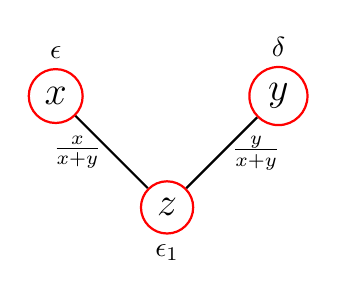
\begin{tikzpicture}[node distance=2cm, mynode/.style={draw=red, thick, circle, font=\Large}]
		\node[mynode, label=below:$\epsilon_1$] (1) {$z$};
		\node[mynode, above left of=1, label=above:$\epsilon$] (2) {$x$};
		\node[mynode, above right of=1, label=above:$\delta$] (3) {$y$};

		\path
		(1) edge[thick] node[left, black] {$\frac{x}{x+y}$} (2)
		(1) edge[thick] node[right, black] {$\frac{y}{x+y}$} (3);
	\end{tikzpicture}
\end{center}
L'errore algoritmico totale sarà dato dalla somma tra gli errori accumulati fino a quel momento su $x$ e $y$
($\epsilon$ e $\delta$) moltiplicati per i coefficiente di amplificazione dovuti all'operazione di somma e l'errore
locale dell'operazione di somma ($\epsilon_1$).

Lo stesso procedimento può essere applicato su $\epsilon$ e $\delta$ per compiere un'analisi più dettagliata di
tali errori.

\subsubsection{Analisi in avanti}
L'\textbf{analisi in avanti} è di norma più pessimista in quanto considera il massimo errore algoritmico
accumulabile.

\begin{example}
	Proviamo a valutare la stabilità di un algoritmo già visto in precendenza, ossia $\frac{x - 1}{x}$.
	\begin{center}
		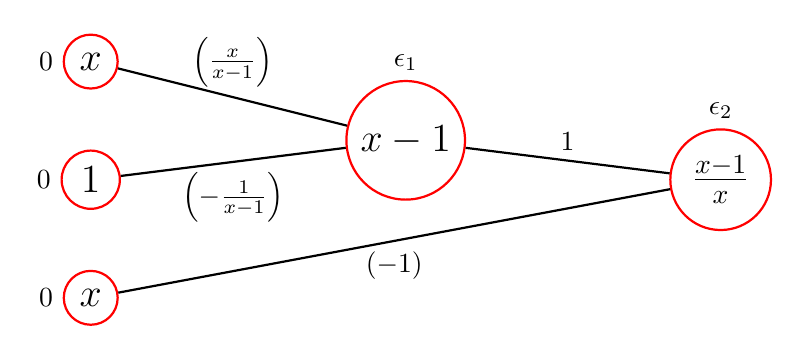
\begin{tikzpicture}[mynode/.style={draw=red, thick, circle, font=\Large}]
			\node[mynode, label=left:$0$] at (0, 1.5) (x1) {$x$};
			\node[mynode, label=left:$0$] at (0, 0) (1) {$1$};
			\node[mynode, label=left:$0$] at (0, -1.5) (x2) {$x$};

			\node[mynode, label=above:$\epsilon_1$] at (4, 0.5) (x-1) {$x-1$};
			\node[mynode, label=above:$\epsilon_2$] at (8, 0) (x-1/x) {$\frac{x-1}{x}$};

			\path
			(x1) edge[thick] node[above, black] {$\left( \frac{x}{x-1} \right)$} (x-1)
			(1) edge[thick] node[below, black] {$\left( -\frac{1}{x-1} \right)$} (x-1)
			(x-1) edge[thick] node[above, black] {$1$} (x-1/x)
			(x2) edge[thick] node[below, black] {$(-1)$} (x-1/x);
		\end{tikzpicture}
	\end{center}
	Dato che stiamo calcolando l'errore algoritmico non mettiamo errore sui dati in ingresso, poiché assumiamo
	che essi siano numeri di macchina (possiamo mettere 0 se preferiamo). L'eventuale errore di rappresentazione
	su tali dati verrà messo in evidenza nel calcolo dell'errore inerente.

	Fatta questa considerazione diventa inutile anche scrivere i coefficienti di amplificazione (scritti comunque
	tra parentesi per completezza) dovuti alle operazioni di sottrazione e divisione (per quanto riguarda il
	denominatore) in quanto verrebbero moltiplicati per 0.

	L'unico coefficiente di amplificazione che ha senso scrivere è quello dovuto all'operazione di divisione (per
	quanto riguarda il numeratore) in quanto andrebbe a moltiplicare l'errore locale $\epsilon_1$ dovuto
	all'operazione di sottrazione.

	Terminiamo scrivendo l'errore locale $\epsilon_2$ dovuto all'operazione di divisione sull'ultimo nodo. L'errore
	algoritmico totale equivale alla quantità
	\begin{align*}
		\ealg = & 0 \cdot \frac{x}{x-1} + 0 \cdot \left( -\frac{1}{x-1} \right) + 0 \cdot (-1) +
		\epsilon_1 \cdot 1 + \epsilon_2                                                          \\
		=       & \epsilon_1 + \epsilon_2
	\end{align*}
	Come in precedenza siamo interessati ad una maggiorazione in valore assoluto dell'errore, ne ricaviamo quindi
	che
	\[ |\ealg| = |\epsilon_1| + |\epsilon_2| \leq 2u \]
	ovvero il risultato ottenuto dall'analisi già fatta in precendenza. Dato che i coefficienti di amplificazione
	che moltiplicano errori non nulli sono costanti, possiamo concludere che l'algoritmo sia numericamente stabile.
\end{example}

\subsubsection{Analisi all'indietro}
In un'\textbf{analisi all'indietro} si assume che il valore calcolato $g(\tx)$ sia uguale, in un'analisi al primo
ordine a $f(\hat{x})$, ossia al valore assunto dalla funzione esatta $f$ valutata su un dato $\hat{x}$ perturbato.
La formula per il calcolo dell'errore algoritmico diventa quindi
\[ \ealg = \frac{f(\hat{x}) - f(\tx)}{f(\tx)} \]
Con questa formula siamo in grado di stimare l'errore algoritmico utilizzando i risultati per l'amplificazione
dell'errore inerente.

Generalmente l'analisi all'indietro conduce a risultati più ottimistici e spesso anche più realistici, andando a
definire la stabilità dell'algoritmo in situazioni di buon condizionamento del problema.
